\documentclass[11pt]{article}
\usepackage[utf8]{inputenc}
\usepackage{geometry}
\usepackage{graphicx}
\usepackage{hyperref}
\usepackage{amsmath}
\usepackage{listings}
\usepackage{xcolor}
\usepackage{float}

% Set page margins
\geometry{a4paper, margin=1in}

% Set up code listing style
\lstset{
    basicstyle=\ttfamily,
    commentstyle=\color{gray},
    keywordstyle=\color{blue},
    stringstyle=\color{red},
    showstringspaces=false,
    captionpos=b
}

\title{Development of a Sudoku Solver: C1 Research Computing Coursework}
\author{Vishal Jain}
\date{\today}

\begin{document}

\maketitle

\tableofcontents

\newpage

\section{Introduction}

\begin{quote}
    "Sudoku is a denial of service attack on human
  intellect" - Ben Laurie
\end{quote}

This report details the development of a Sudoku solver inline with the requirements of the C1 Research Computing coursework. The programme takes as input an incomplete grid in the form of a text file with a 9x9 grid of numbers with zero representing unknown values and `|`,`+`,`-` separating cells and , i.e.:


\begin{verbatim}
    $ cat input.txt
    000|007|000
    000|009|504
    000|050|169
    ---+---+---
    080|000|305
    075|000|290
    406|000|080
    ---+---+---
    762|080|000
    103|900|000
    000|600|000
    \end{verbatim}

and outputs the completed grid in the same form.

\subsection{Background and motivation}

Sudoku, a logic-based combinatorial number-placement puzzle, presents a paradigmatic example of a constraint satisfaction problem (CSP), a class of problems fundamental to the field of computer science. The puzzle's structure, consisting of a 9x9 grid divided into subgrids, adheres to stringent placement rules, thereby embodying the essence of CSPs where the objective is to find a solution that satisfies all given constraints.

This project, centered on the development of a Sudoku solver, is primarily motivated by the pedagogical value inherent in addressing such a well-defined and constrained problem space. Sudoku solvers exemplify the application of algorithmic strategies to a finite, yet non-trivial problem domain. This aligns with the core objectives of the C1 Research Computing coursework, which emphasizes the development of computational solutions that are both efficient and effective.

The logical structure and deterministic nature of Sudoku make it an ideal candidate for exploring various algorithmic approaches, from brute-force methods to more sophisticated heuristic algorithms. Furthermore, the project offers a platform for implementing and refining software development practices, particularly in areas such as code clarity, modular design, and performance optimisation.

In essence, the construction of a Sudoku solver serves not only as an exercise in algorithm implementation but also as a microcosm for broader software development and computational problem-solving skills. It provides a controlled environment to experiment with and evaluate different computational strategies, thereby contributing to a deeper understanding of both the specific problem of Sudoku and the general principles of algorithm design and optimization in computer science.
\section{Problem Decomposition}
To architect the Sudoku solver program, an initial flowchart was constructed to map out the high-level logical sequence. Each step of the flowchart was assigned a color based on its independence; steps that could be altered without impacting preceding steps received a unique color, whereas related, interdependent steps shared the same color. This method helped identify distinct, modular components within the program's workflow. The resulting color-coded flowchart is presented in Figure
\begin{figure}[H]
    \centering
    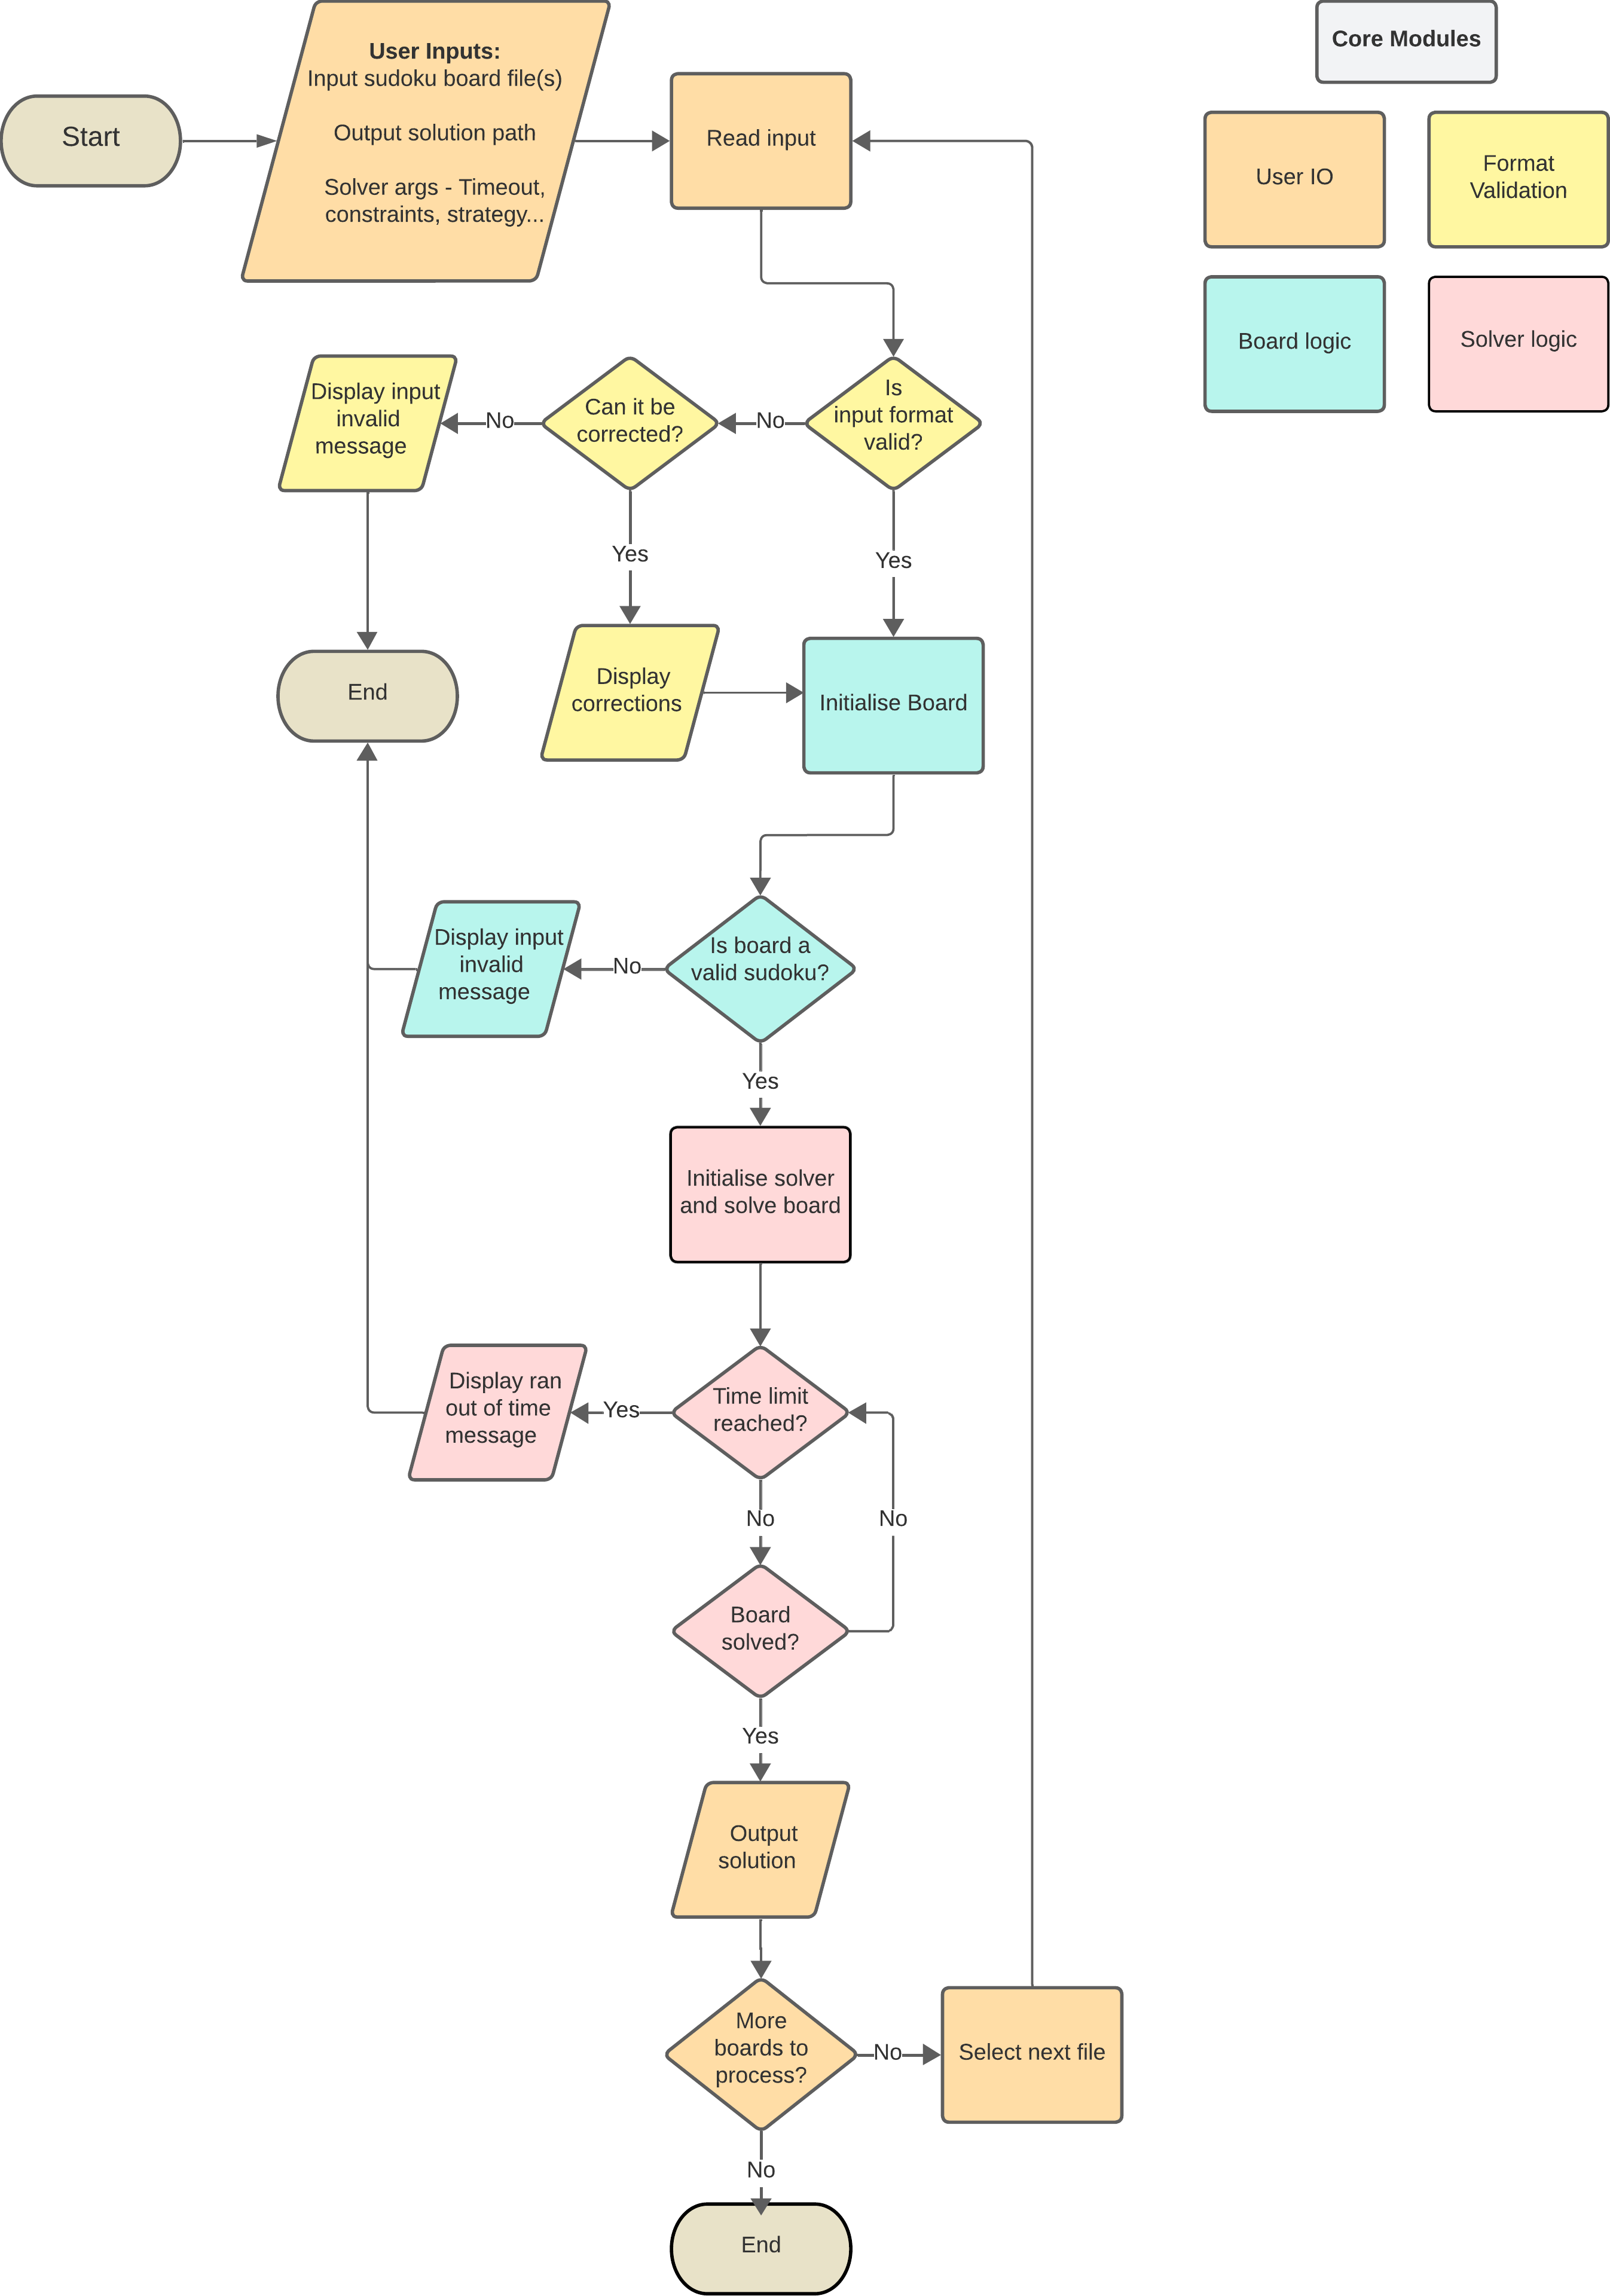
\includegraphics[width=0.82\textwidth]{figs/solver_flowchart.png}
    \caption{High-level flowchart of the Sudoku solver program, illustrating the initial conceptual design. Functionally related modules are color-coded: orange for user interaction, yellow for format validation, cyan for board logic, and pink for solver logic components.}
    \label{fig:solver_flowchart}
\end{figure}
The following modules were identified as the key components of the Sudoku solver:
\begin{itemize}
    \item User IO
    \item Format Validation
    \item Board logic
    \item Solver logic
\end{itemize}
Each module is responsible for error handling of its respective component, and the modules are designed to be as independent as possible. Allowing for the easy replacement of one module with another, as long as the input and output of the module remain the same. This modular design allows for the easy testing of each module and the easy replacement of modules with more efficient ones. The next sections will detail the scope, design, implementation, and limitations of each module, as well as discuss their potential for future development.

\section{User IO}
\subsection{Scope}
The User IO module is responsible for the interaction between the user and the program. It is the only module that interacts with the user, and it is responsible for the following tasks:
\begin{itemize}
    \item Collecting user input.
    \item Validating user input.
    \item Showing the output of the program.
    \item Saving the output of the program.
\end{itemize}

\subsection{Design and Prototyping}
It is ironic that this module which is presented first was actually the last module to be implemented since it required some time spent playing around with the other modules and trying to figure out the best way to call them.

The first step when designing this module for the code was to decide what the requirements were. The requirements were that the user should be able to input a Sudoku board in two ways:
\begin{itemize}
    \item Via a string.
    \item Via a file.

The string input was added because often a new challenging board is recieved online the quickest way to input it is to copy and paste it from the source an

- string input

- collect arguments directly from cli vs passing them through a config

- support

This module represents the main.py script and some functions in utilities.

decision to implement it as functions defined in util and called in main.py vs class

Want to make it easy to run sudokus from the command line, via string or via file. This is because a lot of times you see a board online or someone sends you the board via message so it would be nice to support string input so you could input from clipboard

It will only validate the user input in ways that the fall outside the responsibilities of the other modules. For example, it will check that the user inputs a valid file path, but it will not check that the file contains a valid Sudoku board.

 \dots

this way once changes have been made on the back end, eg a new input file format class is added, a new solver class is added, if the user specifies it, nothing needs to change in main.py

In future, more constraints will be added and solvers will become more complex, taking in more parameters to initialise and having more hyper parameters than just timeout. In which case future extensibility will be important. Add a config file that defines solver and modify main by adding a function to parse this. Rest of the arguments have little scope for extension in the future. At most if a new input format is to be supported it invovles just changing a single line in \dots



% Uncomment the following two lines if you have references
%\bibliographystyle{plain}
%\bibliography{references}

\end{document}
